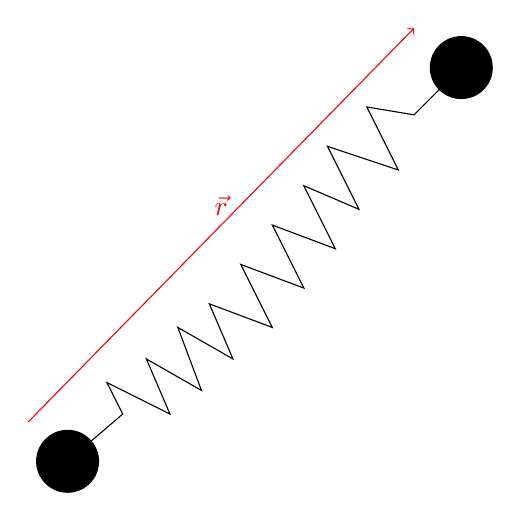
\begin{tikzpicture}
\fill  (0,0) node (v1) {} circle (0.4);
\fill  (5,5) node (v2) {} circle (0.4);

\draw (v1) -- (0.7,0.6) -- (0.5,1) -- (1.3,0.6) -- (1,1.3) -- (1.7,0.9) -- (1.4,1.7) -- (2.1,1.3) -- (1.8,2) -- (2.6,1.7) -- (2.2,2.5) -- (3,2.2) -- (2.6,3) -- (3.4,2.7) -- (3,3.5) -- (3.7,3.2) -- (3.3,4) -- (4.2,3.7) -- (3.8,4.5) -- (4.4,4.4) -- (v2);


\draw [red,->] (-0.5,0.5) -- (4.4,5.5) node [midway,above] {$\vec{r}$};
\end{tikzpicture}